\documentclass[12pt]{article}
\usepackage{braket}
\usepackage{tensor}
\usepackage{fancyhdr}
\usepackage{feynmp-auto}
\usepackage{amsmath,amssymb}
\usepackage{amssymb}
\usepackage{graphicx}
\usepackage{dsfont}
\usepackage{commath}
\usepackage{mathtools}
\usepackage[dutch]{babel}
\usepackage[utf8]{inputenc}
\setlength\parindent{0pt}
\linespread{1.2}
\usepackage[a4paper, total={6.6in, 9in}]{geometry}
\pagestyle{fancy}
\fancyhf{}
\fancyhead[LE,RO]{\slshape \rightmark}
\fancyhead[LO,RE]{\slshape \leftmark}
\fancyfoot[C]{\thepage}
\newcommand{\nucl}[3]{ \ensuremath{ \phantom{\ensuremath{^{#1}_{#2}}} \llap{\ensuremath{^{#1}}} \llap{\ensuremath{_{\rule{0pt}{.75em}#2}}} \mbox{#3} } }
\usepackage{float}

\begin{document}
\def\mean#1{\left< #1 \right>}
\pagenumbering{roman}

\begin{titlepage}

\fontsize{12pt}{14pt}\selectfont

\begin{center}

% Het logo van de Universiteit Gent

\includegraphics[height=3cm]{figuren/ruglogo}

\vspace{1cm}

\fontsize{14pt}{17pt}\selectfont
% De Faculteit:
\textsc{Faculteit Wetenschappen \\ Vakgroep Fysica en Sterrenkunde}
\fontsize{12pt}{14pt}\selectfont
\vspace{0.3cm}

\vspace{1.2cm}

%Het academiejaar: aanpassen!
Academiejaar 2014--2015

\vspace{2.8cm}

\fontsize{17.28pt}{21pt}\selectfont

% De titel van de thesis:
{\textsc{Impulsdistributies voor  atomaire kernen}}

\fontseries{m}
\fontsize{12pt}{14pt}\selectfont

\vspace{3cm}

% De auteur van de thesis:
Jarrick \textsc{Nys}	

\vspace{1.6cm}

% De promotor van de thesis:
Promotor: Prof.~dr.~J.~Ryckebusch\\
Begeleider: Camille~Colle\\

\vspace{2cm}

% De functie van de thesis:
Scriptie voorgedragen tot het behalen van de graad van\\
\textsc{Master in de fysica en sterrenkunde}

\end{center}
\end{titlepage}

\thispagestyle{empty}


\tableofcontents

\newpage

\pagenumbering{arabic}
\section{Inleiding}
\begin{figure}[h!]
\centering
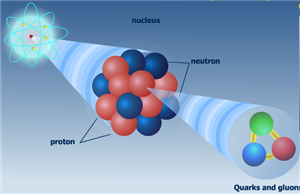
\includegraphics[scale=1]{Atom-Nucleus-Quark}
\end{figure}
Het atoom,  tot begin 19de eeuw bekend als de kleinste bouwsteen van het universum, werd later ontwaard als zijnde een kern met rondom een wolk van elektronen. De kern van een atoom is een zelf-gebonden systeem van nucleonen, waarij we een onderscheid kunnen maken tussen neutronen en protonen.  Het doel van deze thesis is kennis te verwerven over  de eigenschappen van dit systeem en in het bijzonder over de de impuls die de nucleonen bezitten. We bestuderen Impulsdistributies van nulceonen in atomaire kernen. Deze beschrijven hoe de impuls van een nucleon in de kern is verdeeld. Ze kunnen onder meer als input gebruikt worden bij simulaties van scattering experimenten aan nucleonen in een kern. Bij deze experimenten is het nodig om zo goed mogelijk de spectraalfunctie $P(\vec{k},\ E)$ te kennen van de te beschieten kern. De Spectraalfunctie $P(\vec{k},\ E)$ staat in verband met de probabiliteit om een nucleon met impuls $\vec{k}$ te verwijderen waarbij de kern achterblijft met een excitatie-energie $E$. De \'{e}\'{e}ndeeltjes impulsdistributie $n_1(\vec{k})$ kan gerelateerd worden aan de spectraalfunctie via
\begin{equation*}
n^{[1]}(\vec{k}) = \int dE \  P_1(\vec{k},E)
\end{equation*} 
Een voorbeeld van dergelijk experiment is het Long-Baseline Neutrino Experiment (LBNE \cite{anderson2012first}) waar ze gebruik maken van vloeibare-argon detectoren. Een optimale detectie vereist een goede kennis van he het neutrino-argon scatteringproces. Daar \textit{Ankowski et al.}\cite{ankowski2014} meldt dat er geen theoretische studies zijn van de impulsdistributies voor $\nuclide[40][18]{Ar}$ bestuderen hier in het bijzonder deze kern.
We benaderen de nucleus met een gemiddeld-veld model waarbij nucleonen verondersteld worden onafhankelijk van elkaar te bewegen in een sferische symmetrische portentiaal. Correlaties worden dus bij definitie verwaarloosd. De gemiddelde kinetische energie van de neutronen en protonen wordt bepaald aan de hand van de \'{e}\'{e}ndeeltjes momentumdistributie. De tweedeeltjes momentumdistributie wordt bestudeerd in functie van het relatieve momentum, massacentrum momentum en de hoek tussen deze.



\section{E\'{e}ndeeltjes impulsdistributie}
\subsection{Algemene kenmerken}


De kans om een deeltje te vinden met een momentum in het interval $[k,k+dk]$ wordt gegeven door $n_1(k) k^2dk$ waarbij
\begin{equation} \label{eq:one_patricle_distr}
	n_1(\vec{k})=\frac{1}{(2\pi)^3}\int d\vec{r}_1 \int d\vec{r}_1^{\ \prime} e^{i\vec{k}\cdot (\vec{r}_1-\vec{r}^{\ \prime}_1)}\rho_1(\vec{r}_1,\vec{r}_1^{\ \prime}),
\end{equation}
de \'{e}\'{e}ndeeltjes impulsdistributie.

$\rho_1(\vec{r}_1,\vec{r}^{\ \prime}_1)$  stelt de \'{e}\'{e}ndeeltjes niet-diagonale dichtheidsmatrix voor, gedefinieerd als

\begin{equation}
\rho_1(\vec{r}_1,\vec{r}^{\ \prime}_1) = \int \{d\vec{r}_{2-A}\} \Psi^*_A(\vec{r}_1,\vec{r}_2,\vec{r}_3, ... ,\vec{r}_A)\Psi_A(\vec{r}_1^{\ \prime},\vec{r}_2,\vec{r}_3, ... ,\vec{r}_A).
\end{equation}



$\Psi_A(\vec{r}_1,\vec{r}_2,\vec{r}_3, ... ,\vec{r}_A)$ is de grondtoestand van een nucleus met A nucleonen. We maakten gebruik van de volgende notatie

\begin{equation}
\{d\vec{r}_{i-A}\}  = d\vec{r}_i d\vec{r}_{i+1}...\vec{r}_A.
\end{equation}
 


Als $\braket{\Psi_A|\Psi_A}=1$, heeft men dat 


\begin{equation}
\int d\vec{k} \ n_1(\vec{k})= 1.
\end{equation}
Dit is niets anders de totale kans om een deeltje te vinden. Het diagonaalelement $\rho_1(\vec{r},\vec{r})$ stelt de dichtheid van de nucleonen op positie $\vec{r}$ voor.



In het tweedekwantisatie formalisme kan men de  \'{e}\'{e}ndeeltjes momentumdistributie schrijven als
\begin{equation}
n_1(\vec{k})= \frac{1}{A}\bra{\Psi_A} \psi^\dagger(\vec{k}) \psi(\vec{k})\ket{\Psi_A}.
\end{equation}
Intuïtief gezien telt de operator $\psi^\dagger(\vec{k}) \psi(\vec{k})$ het aantal deeltjes met momentum $\vec{k}$. Deze operator wordt voorgesteld in Figuur \ref{fig:feyn}.
\begin{figure} [h]
\centering
\begin{fmffile}{dianpd}
\large % change font size
\boldmath % math in bold
\begin{fmfgraph*}(80,50)
\fmfstraight
\fmfleft{i1,i2,i3,i4,i5,i6}
\fmfright{o1,o2,o3,o4,o5,o6}
\fmf{plain}{i1,v1,o1}
\fmf{plain}{i2,v2,o2}
\fmf{plain}{i3,v3,o3}
\fmf{plain,tension=0.4}{i4,v4}
\fmf{plain,tension=0.4}{v5,o4}
\fmf{fermion,label=$\vec{k}$,label.side=left}{v4,v6}
\fmf{fermion,label=$\vec{k}$, label.side=left}{v7,v5}
\fmfdot{v4,v5}
\fmfforce{(0.3w,1.0h)}{v6}
\fmfforce{(0.7w,1.0h)}{v7}
\fmfforce{(0.3w,0.6h)}{v4}
\fmfforce{(0.7w,0.6h)}{v5}
\end{fmfgraph*}
\end{fmffile}
\caption{Feynman-interpretatie van de  \'{e}\'{e}ndeeltjes momentumoperator. De oprator annihileert en cre\"{e}ert een deeltje met momentum $\vec{k}$ op hetzelfde tijdstip, zo is er geen energiestroom}
\label{fig:feyn}
\end{figure}


Mathematisch kan dit alsvolgt gezien worden:
\begin{align}
n_1(\vec{k}) & =\frac{1}{(2\pi)^3}\int d\vec{r}_1 \int d\vec{r}_1^{\ \prime}\  e^{i\vec{k}\cdot (\vec{r}_1-\vec{r}^{\ \prime}_1)}\rho_1(\vec{r}_1,\vec{r}_1^{\ \prime})  \nonumber \\
& =\int d\vec{r}_1 \int d\vec{r}_1^{\ \prime}  \int d\{\vec{r}_{2-A}\} \braket{\vec{r}_1| \vec{k}} \braket{\vec{k}| \vec{r}_1^{\ \prime}} \braket{\Psi_A | \vec{r}_1, \{ \vec{r}_{2-A}\} } \braket{\vec{r}_1^{\ \prime}, \{ \vec{r}_{2-A}\}|\Psi_A  }   \nonumber \\
& = \frac{1}{A!} \int d\vec{r}_1^{\ \prime}  \int d\{\vec{r}_{2-A}\} \braket{\vec{r}_1| \vec{k}} \braket{\vec{k}| \vec{r}_1^{\ \prime}} \nonumber \\
&\phantom{{aaaa}=3} \times \bra{\Psi_A} \psi^\dagger(\vec{r}_1) \psi^\dagger(\vec{r}_2) \cdots \psi^\dagger(\vec{r}_A) \ket{0} \bra{0} \psi(\vec{r}_A) \cdots \psi(\vec{r}_2) \psi(\vec{r}_1^{\ \prime}) \ket{\Psi_A}
\end{align}
De projectie op de vacuumtoestand $\ket{0} \bra{0}$ kan vervangen worden door de eenheidsoperator omdat $\psi(\vec{r}) \; (\psi^\dagger(\vec{r}))$ reeds alle deeltjes in de ket (bra) vector geannihileerd heeft.
\begin{align}
n_1(\vec{k}) & = \frac{1}{A!} \int d\vec{r}_1^{\ \prime}  \int d{\vec{r}_{2-A}} \braket{\vec{r}_1| \vec{k}} \braket{\vec{k}| \vec{r}_1^{\ \prime}} \nonumber \\
&\phantom{{aaaa}=3} \times \bra{\Psi_A} \psi^\dagger(\vec{r}_1) \psi^\dagger(\vec{r}_2) \cdots \psi^\dagger(\vec{r}_A) \psi(\vec{r}_A) \cdots \psi(\vec{r}_2) \psi(\vec{r}_1^{\ \prime}) \ket{\Psi_A}
\end{align}

Integratie over de coördinaten $\vec{r}_2$ to $\vec{r}_A$ is triviaal aangezien $\int d\vec{r} \psi^\dagger(\vec{r}) \psi(\vec{r})$ de teloperator is in de configuratieruimte. Dus levert de integratie  over  $\vec{r}_A$ een factor  \'{e}\'{e}n omdat het inwerkt op een toestandsvector $\psi(\vec{r}_{A-1}) \cdots \psi(\vec{r}_2) \psi(\vec{r}_1) \ket{\Psi_A}$, waar alle deeltjes, op  \'{e}\'{e}ntje na, geannihileerd zijn. Om dezelfde redenen geeft de integratie over  $\vec{r}_{A-1}$ een factor 2. Als men dus integreert over alle co\"{o}rdinaten $\vec{r}_2$ to $\vec{r}_A$, krijgt men een factor $(A-1)!$.  De  \'{e}\'{e}ndeeltjesmomentumdistributie kan nu geschreven worden als
\begin{align}
n_1(\vec{k}) & = \frac{1}{A}  \int d\vec{r}_1\int d\vec{r}_1^{\ \prime}  \braket{\vec{r}_1| \vec{k}} \braket{\vec{k}| \vec{r}_1^{\ \prime}} \bra{\Psi_A} \psi^\dagger(\vec{r}_1) \psi(\vec{r}_1^{\ \prime}) \ket{\Psi_A}  \nonumber \\
& = \frac{1}{A}  \bra{\Psi_A} \psi^\dagger(\vec{k}) \psi(\vec{k}) \ket{\Psi_A} .
\end{align}
Bij de laatste stap worden de creatie en annihilatieoperatoren in momentumspace gedefini\"{e}erd:
\begin{align}
\psi(\vec{k}) & = \frac{1}{(2\pi)^{3/2}} \int d\vec{r} e^{-i\vec{k} \cdot \vec{r}} \psi(\vec{r})   \nonumber \\
& = \int d\vec{r} \braket{\vec{k}| \vec{r}}  \psi(\vec{r}).
\end{align}

Op een analoge manier kan de niet-diagonale dichtheidsmatrix in het tweedekwantisatie formalisme geschreven worden als
\begin{align}
\rho(\vec{r}_1,\vec{r}^{\ \prime}_1) & =  \int \{d\vec{r}_{2-A}\} \Psi^*_A(\vec{r}_1,\vec{r}_2,\vec{r}_3, ...,\vec{r}_A)\Psi_A(\vec{r}_1^{\ \prime},\vec{r}_2,\vec{r}_3, ... ,\vec{r}_A)   \nonumber \\
& = \frac{1}{A!} \int \{d\vec{r}_{2-A}\} \braket{\Psi_A|\psi^\dagger(\vec{r}_1) \psi^\dagger(\vec{r}_2) ...\psi^\dagger(\vec{r}_A) \psi(\vec{r}_{A-1}) ...  \psi(\vec{r}_2)\psi(\vec{r}_1^{\ \prime})|\Psi_A }  \nonumber  \\
& = \frac{1}{A}\braket{\Psi_A|\psi^\dagger(\vec{r}_1) \psi(\vec{r}_1^{\ \prime})|\Psi_A }.
\end{align}
$\psi^\dagger(\vec{r}_1) \psi(\vec{r}_1^{\ \prime})$ annihileert een deeltje op positie $\vec{r}_1^{\ \prime}$ en cre\"{e}ert een deeltje op positie  $\vec{r}_1$. Intu\"{i}tief telt de diagonaaloperator $\psi^\dagger(\vec{r}_1) \psi(\vec{r}_1)$ het aantal deeltjes op positie $\vec{r}_1$.

\subsection{Het onafhankelijk-deeltjes model}
\subsubsection{Verantwoording}

Dat een onafhankelijk deeltjes model een goede benadering is voor een realistische kern is niet evident. De nucleonen in de kern intrageren namelijk met elkaar via de nucleon-nucleon kracht. Beschouwen we een nucleon-nucleon potentiaal van de vorm
\begin{equation}
V(\vec{r}_1, \vec{r}_2) = V_0 \  f(\vec{r}_1 - \vec{r}_2).
\end{equation}
Hier is $V_0$ de centrale diepte van de potentiaalput en de functie $f$ is van korte dracht en continu. De korte dracht volgt uit de vastelling dat een nucleon niet ingtrageert met alle andere nucleonen in de kern. Dit fenomeen heet saturatie (zie Figuur \ref{fig:bindings_energie}). 
\begin{figure}
\centering 
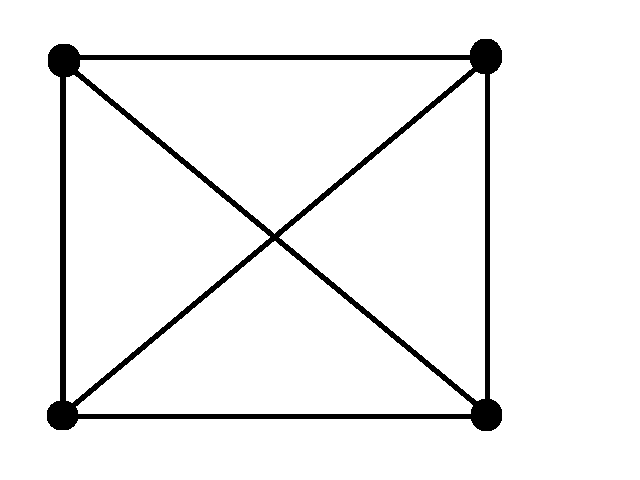
\includegraphics[scale=0.3]{netwerk.png}
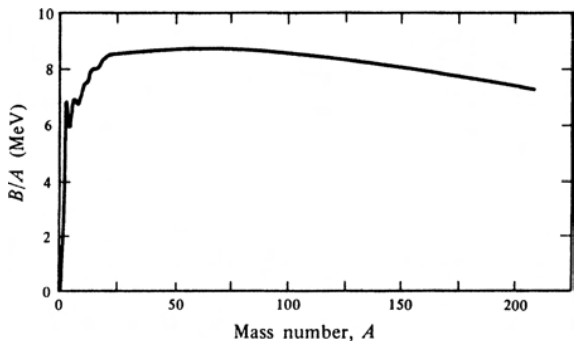
\includegraphics[scale=0.4]{binding_energy.png}
\caption{Links: Beschouwen we een kern met vier nucleonen, $A = 4$. Als elk nucleon met alle andere nucleonen in de kern intrageert dan zijn er $4(4-1)/2$ interacties en is de bindingsenergie ($B$) proportioneel met $A(A-1)$. Voor zware kernen zou dan bij benadering gelden dat $B \propto A^2$ . Rechts: Bindingsenergie per nucleon ($B/A$) als functie van $A$. He tis duidelijk dat een nucleon slechts intrageert met een beperkt aantal andere nucleonen in de kern, m.a.w het aantal interacties per nucleon satureert. Vooral bij zwaardere kernen valt dit op.}
\label{fig:bindings_energie}
\end{figure}
Men kan nu een schatting maken van de centrale potentiaal gevoeld door deeltje 1 door uit te middelen over alle deeltjes intragerend met deeltje 1:
\begin{equation}
V(\vec{r}_1)  = V_0 \int d^3 \vec{r}_2 \ f(\vec{r}_1 - \vec{r}_2) \ \rho (\vec{r}_2).
\end{equation}
Als de dracht van $f$ kort genoeg is kan $\rho (\vec{r}_2)$ benaderd worden door $\rho (\vec{r}_1)$. $V(\vec{r}_1)$ wordt dan
\begin{equation}
V(\vec{r}_1)  = C\  V_0  \ \rho (\vec{r}_1).
\end{equation} 
We weten dus dat de potentiaal gevoeld door een deeltje in de kern bij benadering everedig is met de dichtheidsdistributie van de kern. Uit \cite{povh2008particles} weten we dat een Fermi functie een goede benadering is voor de dichtheidsdistributie van een kern:
\begin{equation}
\rho (r) = \frac{\rho (0)}{1+\exp{(r-c)/a}}.
\end{equation}
Hier is $c$ de straal is waarbij de distributie de helft is van zijn maximale waarde en $a$ de spreiding waarover de distributie afneemt.
Men krijgt dan de Wood-Saxon potentiaal \cite{povh2008particles}
\begin{equation}
V(\vec{r}_1)  = \frac{C\  V_0  \ \rho (0)}{1+\exp{(r-c)/a}}.
\end{equation}
De Schr\"{o}dingervergelijking voor dergelijke potentiaal heeft geen analytische oplossing dus trachten we de potentiaal te benaderen met een sferische harmonische oscillator potentiaal
\begin{equation}
V_{HO}(r) = \frac{1}{2} M_N \omega^2 r^2,
\end{equation}
met de volgende parametrisatie van $\hbar \omega$:
\begin{equation}
\hbar\omega (MeV) = 45A^{-1/3}-25A^{-2/3},
\end{equation}
Figuur \ref{fig:hows} laat zien dat dit een relatief goede benadering is. 

\begin{figure}
\centering
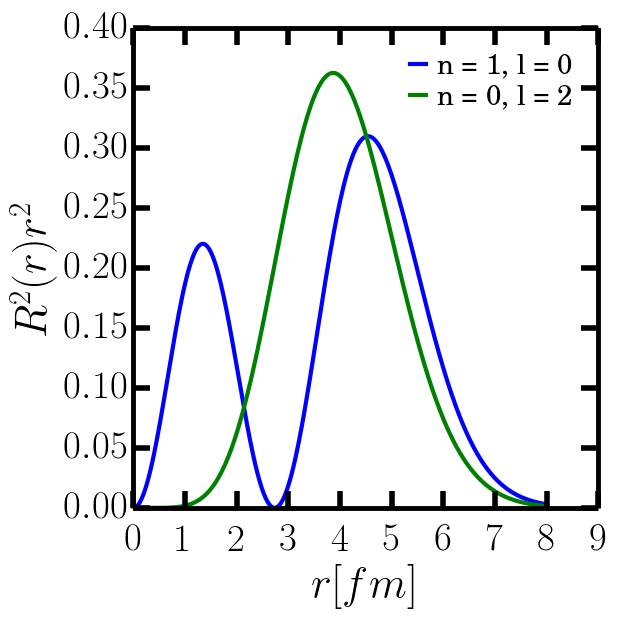
\includegraphics[scale=0.5]{waves.png}
\caption{probabiliteitsdistributie voor twee ontaarde toestanden in harmonische oscillator  ($N =2$)}
\label{fig:ho_waves}
\end{figure}

\begin{figure}
\centering
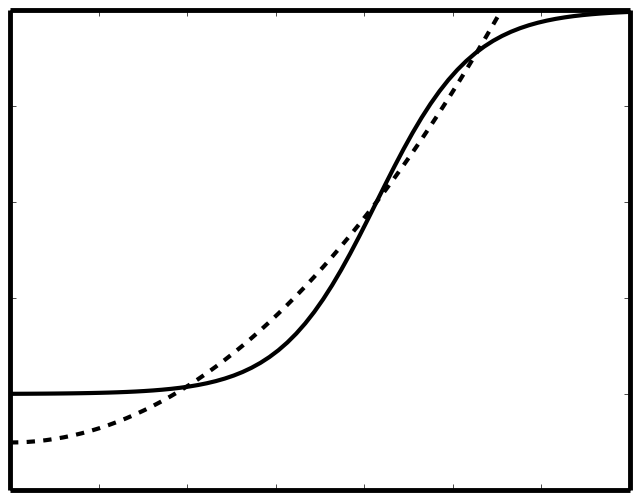
\includegraphics[scale=0.4]{Ar_potentiaal.png}
\caption{De volle curve is een Wood-Saxon potentiaal en de gestreepte curve deze van een harmonische oscillator.}
\label{fig:hows}
\end{figure}



\subsubsection{Oplossen van de Schr\"{o}dingervergelijking voor een sferische harmonische oscillator potentiaal}
Beschouw nucleonen die onafhankelijk van elkaar in een sferische harmonische osciallor potentiaal bewegen, beter bekend als de gemiddeld-veld benadering (GV). De Hamiltoniaan vereenvoudigt dan tot
\begin{equation}
\hat{H} = \sum_i^A \hat{T}_i + \sum_{\substack{ij \\ i  \neq j}}^A \hat{V}_{ij}  + \sum_{\substack{klm \\ k \neq l \neq m}}^A \hat{W}_{klm} \xrightarrow{GV} \hat{H} = \sum_i^A \left(\hat{T}_i + \hat{V}_i \right)
\end{equation}
De nieuwe hamiltionaan is slechts een som van \'{e}\'{e}ndeeltjes-Hamiltonianen, met andere woorden het probleem reduceert zicht tot een \'{e}\'{e}ndeeltjesprobleem:
\begin{equation} \label{eq:HO}
\left( -\frac{\hbar^2}{2M_N} \nabla^2 + \frac{1}{2} M_N \omega^2 r^2 \right) \psi_{nlm}(\vec{r}) = E\psi_{nlm}(\vec{r}).
\end{equation}
$\hbar\omega$ kan alsvolgt geparametriseerd worden
\begin{equation}
\hbar\omega (MeV) = 45A^{-1/3}-25A^{-2/3},
\end{equation}
waarbij $A$ het aantal nucleonen is in de kern. Een eigenfunctie van vergelijking (\ref{eq:HO}) wordt gegeven door
\begin{equation} \label{eq:solution_ho}
\psi_{nlm}(\vec{r}) \equiv \braket{\vec{r}|nlm} = R_{nl}(r)Y_{lm}(\Omega)	
\end{equation}
waar $Y_{lm}(\Omega)$ de sferische harmonieken voorstelt. Het radi\"{e}le deel van de golffunctie in functie van de gegeneraliseerde Laguerre-polynomen $L^\alpha_n(r)$ wordt gegeven door
\begin{equation}
 R_{nl}(r) = \left[ \frac{2n!}{\Gamma(n+l+\frac{3}{2})}\nu^{l+\frac{3}{2}} \right]^{\frac{1}{2}} r^l e^{-\frac{\nu r^2}{2}} L^{l+\frac{1}{2}}_n(\nu r^2)
\end{equation}
waar
\begin{equation}
\nu \equiv \frac{M_N \omega}{\hbar}.
\end{equation}

De energie eigenwaarden zijn zijn onafhankelijk van $m_l$ als gevolg van de sferische symmetrie:
\begin{equation}
E_{nl} = \hbar \omega \left(2n+ l_ + \frac{3}{2} \right)
\end{equation} 

Nadelig aan de harmonische oscillator potentiaal is de eigenaardige ontaarding van de energieniveaus. Deze ontaarding is er namelijk niet bij een Wood-Saxon potentaal. Bijvoorbeeld, toestanden $2s$ en $1d$  hebben dezelfe energie. We gebruiken de opvulling van een Wood-Saxon om bij het opvullen van de toestand deze vervelende ontaarding te vermijden. Hoe gebeurt de de opvulling dan?  Figuur \ref{fig:ho_waves} geeft aan dat toestanden van de harmonische oscillator in met een hoger impulsmoment $l$ zich met grotere  waarschijnlijkheid verder van het centrum kern begeven dan toestanden met kleinere $l$. De realistische potentiaal is dieper op grote afstand en minder diep op kleine afstand van het centrum dan de harmonische oscillator potentiaal. Dus toestanden met grote $l$ voelen een diepere potentiaal en schuiven dus naar lagere energie\"{e}n. 



\subsubsection{E\'{e}ndeeltjes impulsdistributie in een harminsche oscillator potentiaal}
Een onafhankelijk deeltjes model (IPM) veronderstelt een nucleon beweegt in het gemiddelde veld van alle andere nucleonen. De totale golffunctie van de nucleus is dus een Slaterdeterminant is van de \'{e}\'{e}ndeeltjes golffuncties:

\begin{equation} \label{eq:slater}
\Psi_A(\vec{r}_1,\vec{r}_2,\vec{r}_3, ... ,\vec{r}_A)= \frac{1}{\sqrt{A!}} \sum^A_{\substack{i_1 i_2 \ldots i_A}} 
													  \varepsilon_{i_1 i_2 \ldots i_A} \phi_{i_1}(\vec{r}_1)
													         \phi_{i_2}(\vec{r}_2)...
													         \phi_{i_A}(\vec{r}_A).
\end{equation}

$\varepsilon_{i_1 i_2 \ldots i_A}$ staat voor het totaal ant-symmetrische Levi-Civita tensor en de sommaties over de indices $i_1,\ldots ,i_A$  gaan van \'{e}\'{e}n tot A. De \'{e}\'{e}ndeeltjes golffuncties voldoen aan de orthonormaliteitsregel:

\begin{equation} \label{eq:orthogonality}
\int d\vec{r}_i \phi^*_l(\vec{r}_i)\phi_m(\vec{r}_i) = \delta_{lm}.
\end{equation}

Gebruik makende van deze eigenschap wordt de \'{e}\'{e}ndeeltjes niet-diagonale matrix 

\begin{align}
\rho_1(\vec{r}_1,\vec{r}^{\ \prime}_1) 
&  = \frac{1}{A!} 	 \sum_{\substack{i_1 i_2 \ldots i_A}} \sum_{\substack{j_1j_2 \ldots j_A}} \varepsilon_{i_1 i_2 \ldots i_A} \varepsilon_{j_1j_2 \ldots j_A} \phi^*_{i_1}(\vec{r}_1) \phi_{j_1}(\vec{r}_1^{\ \prime}) 
\delta_{i_2,j_2}\delta_{i_3,j_3}...\delta_{i_A,j_A}  \nonumber \\
& = \frac{1}{A}\sum_{\substack{i}} \phi^*_i(\vec{r}_1) \phi_i(\vec{r}_1^{\ \prime}).
\end{align}

en met  de definitie van de golffunctie in de impulsruimte:
\begin{equation}
\phi_i(\vec{k}) = \frac{1}{(2\pi)^{3/2}} \int d\vec{r} e^{-i\vec{k}\cdot \vec{r}} \phi_i(\vec{r})
\end{equation}
wordt \eqref{eq:one_patricle_distr}:
\begin{align} 
	n^{[1]}(\vec{k})&=\frac{1}{A(2\pi)^3} \sum_{\substack{i}} \int d\vec{r}_1 \int d\vec{r}_1^{\ \prime} e^{i\vec{k}\cdot (\vec{r}_1-\vec{r}^{\ \prime}_1)}
	\phi^*_i(\vec{r}_1)\phi_i(\vec{r}_1^{\ \prime})\nonumber \\
	& = \frac{1}{A} \sum_{\substack{i}} \phi^*_i(\vec{k})\ \phi_i(\vec{k}) \nonumber\\
	& = \frac{1}{A} \sum_{\substack{i}} \ \abs{\phi_i(\vec{k}) }^2.
\end{align}
De golffuncties in de impulsruimte krijgen we door de Schr\"{o}dinger vergelijking (\ref{eq:HO}) in de impulsruimte,
\begin{equation} \label{eq:HO_momentum}
\left( -\frac{M_N \omega^2}{2} \nabla^2 + \frac{\hbar^2}{2M_N} k^2 \right) \tilde{\psi}_{nlm}(\vec{k}) = E\tilde{\psi}_{nlm}(\vec{k}),
\end{equation}
op te lossen. Deze diiferentiaalvergelijking heeft de zelfde vorm als de Schr\"{o}dinger vergelijking in de configuatieruimte, met andere woorden de oplossingen zijn van dezelfde vorm als \ref{eq:solution_ho}
\begin{equation}
\psi_{nlm}(\vec{k}) \equiv \braket{\vec{k}|nlm} = K_{nl}(k)Y_{lm}(\Omega_k)	
\end{equation}
met
\begin{equation}
 K_{nl}(k) = \left[ \frac{2n!}{\Gamma(n+l+\frac{3}{2})}\nu'^{l+\frac{3}{2}} \right]^{\frac{1}{2}} k^l e^{-\frac{\nu' k^2}{2}} L^{l+\frac{1}{2}}_n(\nu' k^2)
\end{equation}
en
\begin{equation}
\nu^{\ \prime} \equiv \frac{\hbar}{M_N \omega}.
\end{equation}

De totale golffunctie in impulsruimte van een deeltje in een sferische harmonische oscillatorpotentiaal wordt gegeven door
\begin{equation}
\phi_\alpha (\vec{k}) = \psi_{n_\alpha l_\alpha m_\alpha}(\vec{k}) \chi_{\frac{1}{2}\sigma_\alpha}  \xi_{\frac{1}{2}\tau_\alpha}.
\end{equation}
$\chi_{\frac{1}{2}\sigma_\alpha} $ en $\xi_{\frac{1}{2}\tau_\alpha}$ zijn respectievelijk de abstracte spin- en isospintoestand waarbij de eerste index steeds de spin- of isospinvector voorstelt en de tweede index de projectie.

Omdat de potentiaal sferisch symmetrisch is kan men de momentum golffunctie factoriseren in een hoekafhankelijk deel en een radi\"{e}el deel. Als men naar de distributie van de grootte van het momentum wil kijken kan men integreren over alle hoekafhankelijkheid $\Omega_k$, dit leidt dan tot
\begin{align}
n_1(k) &  =  \frac{1}{A} \int d\Omega_k \sum_{\tau nlm\sigma}\ \psi^*_{n l m}(\vec{k})\psi_{n l m}(\vec{k}) \ \chi^*_{\frac{1}{2}\sigma} \chi_{\frac{1}{2}\sigma}\ \xi^*_{\frac{1}{2}\tau}  \xi_{\frac{1}{2}\tau} \nonumber\\
& =  \frac{1}{A} \sum_{\tau nlm\sigma }K^2_{nl}(k)\ \chi^*_{\frac{1}{2}\sigma} \chi_{\frac{1}{2}\sigma} \ \xi^*_{\frac{1}{2}\tau}  \xi_{\frac{1}{2}\tau}.
\end{align}
De bovengrenzen van sommaties over $n,l,m,\sigma$ hangen af van het aantal protonen ($\tau =+1/2$) en neutronen  ($\tau =-1/2$) in de beschouwde kern.

\subsection{Resultaten}

De \'{e}\'{e}ndeeltjes impulsdistributies voor veschillende kernen worden getoond in Figuur \ref{fig:oneparticledistr}. De distributies zijn op \'{e}\'{e}n genormeerd. Zoals verwacht wordt $n^{[1]}(k)$ heel klein voor $k$ gaande naar oneindig. We kunnen nu de gemiddelde kinetische energie bepalen van een nucleon in een kern:
\begin{equation}\label{eq:kin}
\mean{T_N} = \frac{\hbar^2}{2M_N} \int dk\ n_N^{[1]}(k)\ k^4.
\end{equation}
De index $N$ kan $n$ (neutron) of $p$ (proton) zijn. $n_N^{[1]}(k)$ stelt de \'{e}\'{e}ndeeltjes impulsdistributie van de neutronen of protonen afhankelijk van de index $N$. Resultaten voor de kinetische enrgie \ref{eq:kin} zijn te vinden in Tabel \ref{tab:kineticenergy}. Uit \cite{maarten} blijkt dat de gemiddeld-veld benadering goed is bij lage impuls maar naarmate we naar grotere impuls gaan zorgen correlaties voor een grote staart. De kinetische energie is gerelateerd aan het vierde moment van de momentum distributie en daarom dus sterk afhankelijk van de staart van de distributie. Correlaties tussen de nucleonen zorgen dus voor een enorme toename in gemiddelde kinetische energie.

\begin{figure}[h!]
\centering
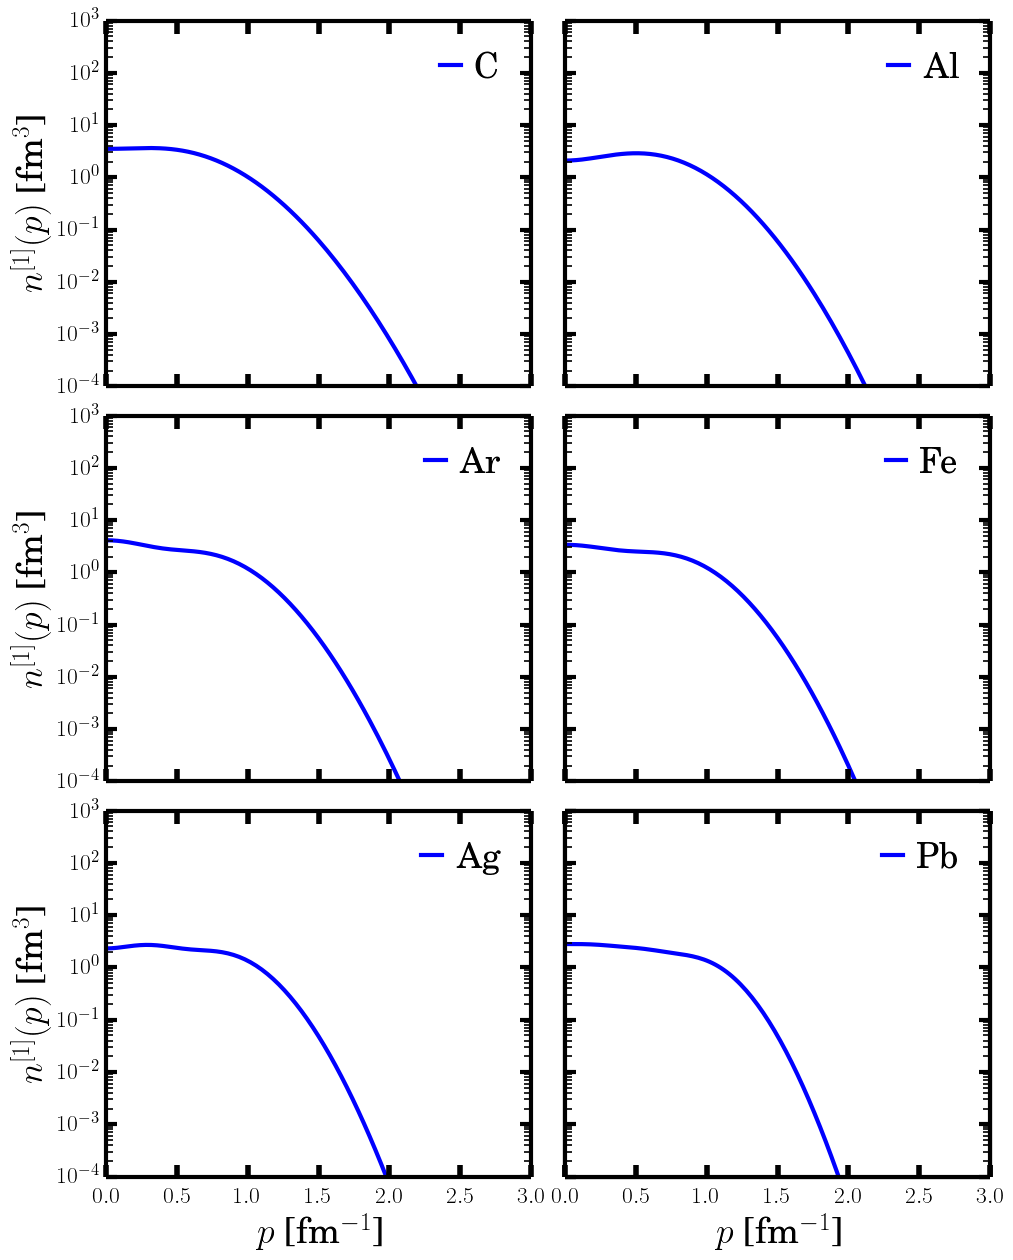
\includegraphics[scale=0.6]{multi.png}
\caption{$n^{[1]}(k)$ voor $\nuclide[4][2]{He}, \nuclide[27][13]{Al},\nuclide[40][18]{Ar},\nuclide[56][26]{Fe}, \nuclide[109][47]{Ag}, \nuclide[208][82]{Pb} $.}
\label{fig:oneparticledistr}
\end{figure}

\begin{table}
\centering
\begin{tabular}{cc | cc}
$A$ & $x_p$ &  $\mean{T_p}\ (MeV)$ & $\mean{T_n}\ (MeV)$ \\
\hline
\hline
$\nuclide[4][]{He}$ & $0.500$&$13.82$ &$13.82$ \\
$\nuclide[9][]{Be}$ &$0.444$& $15.86$ &	$16.65$ \\
$\nuclide[12][]{C}$ &$0.500$ &$16.13$	& $16.13$ \\
$\nuclide[16][]{O}$ &$0.500$ &$15.66$	& $15.66$ \\
$\nuclide[27][]{Al}$ &$0.481$ &$16.69$ 	& $17.02$ \\
$\nuclide[40][]{Ar}$&$0.450$ &$16.22$	& $17.28$ \\
$\nuclide[40][]{Ca}$ &$0.500$& $16.53$ &	$16.53$ \\
$\nuclide[48][]{Ca}$ &$0.417$ &$15.73$	& $17.98$ \\
$\nuclide[56][]{Fe}$ & $0.464$&$16.82$	& $17.59$ \\
$\nuclide[108][]{Ag}$&$0.435$& $16.74$	& $18.17$ \\ 
$\nuclide[208][]{Pb}$&$0.394$ &$16.49$	& $18.93$ \\
\end{tabular}
\caption{De gemiddelde kinetische energie van neutronen en protonen voor verschillende kernen. $x_p$ is de protonfractie $x_p = Z/A$.}
\label{tab:kineticenergy}
\end{table}


\section{Tweedeeltjes impulsdistributie}
\subsection{Algemene kenmerken}
De kans om een deeltje met impuls in het interval $[k_1,k_1+dk_1]$ te vinden wanneer een ander deeltje een impuls heeft in het interval $[k_2,k_2+dk_2]$ wordt gegeven door $ n_2(k_1,k_2)dk_1dk_2$ met

\begin{equation}
n_2(\vec{k}_1,\vec{k}_2)=\frac{1}{(2\pi)^6}\int d\vec{r}_1 \int d\vec{r}_2 \int  
    						d\vec{r}_1^{\ \prime} \int d\vec{r}_2^{\ \prime} 
    						\mathrm{e}^{i\vec{k}_1\cdot (\vec{r}_1-\vec{r}^{\ \prime}_1)} 
    						\mathrm{e}^{i\vec{k}_2\cdot(\vec{r}_2-\vec{r}^{\ \prime}_2)}
    						\rho_2(\vec{r}_1,\vec{r}_2; \vec{r}_1^{\ \prime},\vec{r}_2^{\ \prime})
\end{equation}
de tweedeeltjes impulsdistributie. Hier stelt 


\begin{equation}
\rho_2(\vec{r}_1,\vec{r}_2, \vec{r}_1^{\ \prime},\vec{r}_2^{\ \prime}) = \int \{d\vec{r}_{3-A}\} \Psi^*_A(\vec{r}_1,\vec{r}_2,\vec{r}_3, ... ,\vec{r}_A)\Psi_A(\vec{r}_1^{\ \prime},\vec{r}_2^{\ \prime},\vec{r}_3, ... ,\vec{r}_A)
\end{equation}

de tweedeeltjes niet-diagonale dichtheidsmatrix voor.

Het interessant deze te bestuderen in functie van relatieve ($\vec{r}$) en massacentrumcoordinaten ($\vec{R}$), een natuurlijker co\"{o}rdinatensysteem voor twee deeltjes (Figuur \ref{fig:coordinates}):

\begin{figure}
\centering
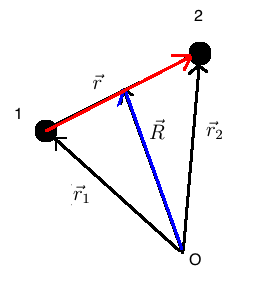
\includegraphics[scale=0.6]{coordinates.png}
\caption{ Illustratie van relatieve en massacentrum coordinaten.}
\label{fig:coordinates}
\end{figure}
\begin{equation}
\vec{r}= \frac{1}{\sqrt{2}} \left(\vec{r}_1 - \vec{r}_2\right)  \qquad \vec{R}= \frac{1}{\sqrt{2}} \left(\vec{r}_1 + \vec{r}_2\right)
\end{equation}

Dan transformeren de impulsco\"{o}rdinaten alsvolgt:
\begin{equation}
\vec{k}= \frac{1}{\sqrt{2}} \left(\vec{k}_1 - \vec{k}_2\right) \qquad \vec{P}= \frac{1}{\sqrt{2}} \left(\vec{k}_1 + \vec{k}_2\right)
\end{equation}
En wordt de tweedeeltjes impulsdistributie in functie van deze neiuwe co\"{o}rdinaten:
\begin{equation}
n(\vec{k},\vec{P})=\frac{1}{(2\pi)^6}
						\int d\vec{r} \int d\vec{R} \int d\vec{r}^{\ \prime} \int d\vec{R}^{\ \prime} 
    						\mathrm{e}^{i\vec{k}\cdot (\vec{r}-\vec{r}^{\ \prime})} 
    						\mathrm{e}^{i\vec{P}\cdot(\vec{R}-\vec{R}^{\ \prime})} 
    						\rho_2(\vec{r},\vec{R}; \vec{r}^{\ \prime},\vec{R}^{\ \prime})
\end{equation}

met

\begin{equation} \label{eq:twobodydensity}
\rho_2(\vec{r},\vec{R}; \vec{r}^{\ \prime},\vec{R}^{\ \prime}) = 
							\rho_2\left(	
							\vec{r}_1=\frac{\vec{r} + \vec{R}}{\sqrt{2}},
							\vec{r}_2=\frac{-\vec{r} + \vec{R}}{\sqrt{2}},
						    \vec{r}_1^{\ \prime}=\frac{\vec{r}^{\ \prime} + \vec{R}^{\ \prime}}{\sqrt{2}},	
						    \vec{r}_2^{\ \prime}=\frac{-\vec{r}^{\ \prime} + \vec{R}^{\ \prime}}{\sqrt{2}}
						    \right)
\end{equation}

De tweedeeltjes impulsdsitributie kan in het tweedekwantisatie formalisme geschreven worden als

\begin{equation}
\label{eq:2BNDM}
n_2(\vec{k_1},\vec{k_2})= \frac{1}{A(A-1)}\bra{\Psi_A} \psi^\dagger(\vec{k}_1) \psi^\dagger(\vec{k}_2)  \psi(\vec{k}_1)  \psi(\vec{k}_2)  \ket{\Psi_A}
\end{equation}
en de tweedeeltjes niet-diagonale dichtheidsmatrix als
\begin{align}
\rho(\vec{r}_1, \vec{r}_2; \vec{r}_1^{\ \prime}, \vec{r}_2^{\ \prime}) & =  \int \{d\vec{r}_{3-A}\} \Psi^*_A(\vec{r}_1,\vec{r}_2,\vec{r}_3, ... ,\vec{r}_A)\Psi_A(\vec{r}_1^{\ \prime},\vec{r}_2^{\ \prime},\vec{r}_3, ... ,\vec{r}_A)  \nonumber\\
& = \frac{1}{A!} \int \{d\vec{r}_{3-A}\} \braket{\Psi_A | \psi^\dagger(\vec{r}_1) \psi^\dagger(\vec{r}_2)\psi^\dagger(\vec{r}_3) ...\psi^\dagger(\vec{r}_A) \psi(\vec{r}_A) ...\psi(\vec{r}_3)\psi(\vec{r}^{\ \prime}_2) \psi(\vec{r}^{\ \prime}_1)|\Psi_A } \nonumber \\
& = \frac{1}{A(A-1)} \braket{\Psi_A | \psi^\dagger(\vec{r}_1) \psi^\dagger(\vec{r}_2)\psi(\vec{r}^{\ \prime}_2) \psi(\vec{r}^{\ \prime}_1)|\Psi_A }. 
\end{align}
De operator in \eqref{eq:2BNDM} telt het aantal deeltjes met impuls $\vec{k}_1$ en impuls $\vec{k}_2$.



\subsection{Het onafhankelijk-deeltjes model}


Een uitdrukking voor de tweedeeltjes niet-diagonale matrix kan men bekomen door  (\ref{eq:twobodydensity}) uit te rekenen waarbij de totale golffunctie van de nucleus een de Slaterdeterminant (\ref{eq:slater}) is. Rekening houdend met de orthogonaliteitsrelatie (\ref{eq:orthogonality}) vindt men 

\begin{align}
\rho_2(\vec{r}_1,\vec{r}_2;\vec{r}^{\ \prime}_1,\vec{r}^{\ \prime}_2) 
&  = \frac{1}{A!} 	 \sum_{\substack{i_1 i_2 \ldots i_A}} \sum_{\substack{j_1j_2 \ldots j_A}} \varepsilon_{i_1 i_2 \ldots i_A} \varepsilon_{j_1j_2 \ldots j_A} \phi^*_{i_1}(\vec{r}_1)\phi^*_{i_2}(\vec{r}_2) \phi_{j_1}(\vec{r}_1^{\ \prime})\phi_{j_2}(\vec{r}_2^{\ \prime})
\delta_{i_3,j_3}...\delta_{i_A,j_A} \nonumber \\
&  = \frac{1}{A(A-1)} 	 \sum_{\substack{i_1 i_2}} \sum_{\substack{j_1j_2}} \left(\delta_{i_1j_1}\delta_{i_2j_2} - \delta_{i_1j_2}\delta_{i_2j_1} \right)
\phi^*_{i_1}(\vec{r}_1)\phi^*_{i_2}(\vec{r}_2) \phi_{j_1}(\vec{r}_1^{\ \prime})\phi_{j_2}(\vec{r}_2^{\ \prime}) \nonumber \\
& = \frac{1}{A(A-1)}\sum_{\substack{i j}} \left[\phi^*_{i}(\vec{r}_1)\phi^*_{j}(\vec{r}_2) \phi_{i}(\vec{r}_1^{\ \prime})\phi_{j}(\vec{r}_2^{\ \prime})  - \phi^*_{i}(\vec{r}_1)\phi^*_{j}(\vec{r}_2) \phi_{j}(\vec{r}_1^{\ \prime})\phi_{i}(\vec{r}_2^{\ \prime}) \right].
\end{align}

Dan kan de tweedeeltjes momentumdistributie alsvolgt geschreven worden:

\begin{align} \label{two-body}
n_2(\vec{k}_1,\vec{k}_2) & = \frac{1}{A(A-1)}\sum_{\substack{i j}} \left[\phi^*_{i}(\vec{k}_1)\phi^*_{j}(\vec{k}_2) \right] \left[ \phi_{i}(\vec{k}_1)\phi_{j}(\vec{k}_2)  - \phi_{j}(\vec{k}_1)\phi_{i}(\vec{k}_2) \right] \nonumber  \\
& = \frac{1}{2A(A-1)}\sum_{\substack{i j}} \left[\phi^*_{i}(\vec{k}_1)\phi^*_{j}(\vec{k}_2)- \phi^*_{j}(\vec{k}_1)\phi^*_{i}(\vec{k}_2) \right] \left[ \phi_{i}(\vec{k}_1)\phi_{j}(\vec{k}_2) - \phi_{j}(\vec{k}_1)\phi_{i}(\vec{k}_2) \right].
\end{align}

\subsubsection{Twee-deeltjes momentumdistributies in relatieve- massacentrumcoordinaten}

De positie van twee deeltjes kan beschreven worden door een vector van het centrum van de potentiaalput naar elk van de deeltjes, namelijk $\vec{r}_1$ en $\vec{r}_2$. Twee deeltjes kunnen ook beschreven worden door een relatieve co\"{o}rdinaat $\vec{r}$ en een co\"{o}rdinaat $\vec{R}$ die de positie van het massacentrum van de twee deeltjes beschrijft. De golffunctie van een tweedeeltjes systeem in de co\"{o}rdinatenruimte kan bijgevolg op twee manieren worden geschreven, namelijk als $\braket{\vec{r}_1|n_1 l_1 m_1}\braket{\vec{r}_2 | n_2 l_2 m_2}$ of als $\braket{\vec{r}| n l m}\braket{\vec{R} | NLM}$. Voor een harmonische oscillator potentiaal blijft de vorm van de golffuncties identiek maar veranderen de kwantumgetallen. In het nieuwe co\"{o}rdinatensysteem worden de kwantumgetallen $n,\  l$  en $N,\ L$. De eerste twee beschrijven de relatieve beweging van de deeltjes en de laatste beschrijven de beweging van het massacentrum.  Men kan $l_1,\  l_2$  en $l,\  L$ koppelen tot een totaal impulsmoment $L$. 
\begin{align}
& \left| l_1-l_2 \right| \leq \Lambda \leq l_1 + l_2 \\
& \left| l-L \right| \leq \Lambda \leq l+ L
\end{align}

Twee deeltjes zijn gekoppeld tot een welbepaald impulsmoment $\Lambda$ en projectie $M_\Lambda$
\begin{align}
&\Ket{n_1l_1n_2l_2;\Lambda M_\Lambda} = \sum_{m_1, m_2} \Ket{n_1l_1m_1n_2l_2m_2} \Braket{l_1m_1,l_2m_2| \Lambda M_\Lambda} \\
&\Ket{nlNL;\Lambda M_\Lambda} = \sum_{m, M} \Ket{nlm NLM} \Braket{lm LM|\Lambda M_\Lambda} 
\end{align}
Een harmonische oscillator tweedeeltjes golfunctie met totaal impulsmoment $\Lambda$  en projectie $M_\Lambda$ heeft een orthogonale transformatie van individuele co\"{o}rdinaten naar relatieve en massacentrumco\"{o}rdinaten
\begin{align} \label{eq:moshinsky_trans}
\Ket{n_1l_1n_2l_2;\Lambda M_\Lambda} = \sum_{nl, N\Lambda} \Ket{nlNL;\Lambda M_\Lambda} \Braket{nlNL;\Lambda | n_1l_1n_2l_2;\Lambda}.
\end{align}
De transformaticoeffici\"{e}nten $\Braket{nlNL;\Lambda | n_1l_1n_2l_2;\Lambda}$ zijn gekend als de Moshinsky brackets. Deze zijn onafhankelijk van $M_\Lambda$. De energie van een deeltje ( $E$) in een harmonische oscillator potentiaal  is $\hbar\omega  (2n_1+l_1+ \frac{3}{2})$. De totale energie van twee deeltjes moet dezelfde zijn in beide co\"{o}rdinatensystemen
\begin{equation}
2n_1 + l_1 + 2n_2 + l_2 = 2n + l + 2N + L
\end{equation}
De Moshinsky brackets zijn gelijk aan nul als deze gelijkheid niet is voldaan. 


\subsubsection{Tweedeeltjes momentumdistributie met HO potentiaal}
Tweedeeltjes momentumdistributie in centraal co\"{o}rdinatensysteem wordt gegeven door:
\begin{align} \label{eq:two-body}
n_2(\vec{k}_1,\vec{k}_2) = \frac{1}{2A(A-1)}\sum_{\substack{\alpha \beta \\ \alpha  \neq \beta}} \left[\phi^*_{\alpha}(\vec{k}_1)\phi^*_{\beta}(\vec{k}_2)- \phi^*_{\beta}(\vec{k}_1)\phi^*_{\alpha}(\vec{k}_2) \right] \left[ \phi_{\alpha}(\vec{k}_1)\phi_{\beta}(\vec{k}_2)  - \phi_{\beta}(\vec{k}_1)\phi_{\alpha}(\vec{k}_2) \right].
\end{align}
De sommatie gaat over alle bezette toestanden in de kern ($n_\gamma$, $l_\gamma$, $m_\gamma$, $\sigma_\gamma$, $\tau_\gamma$). We willen deze nu schrijven in functie van $\vec{k}$ en $\vec{P}$.
Beschouw het product van twee golffuncties in impulsruimte:
\begin{equation} \label{eq:wave_two}
\psi_{n_\alpha l_\alpha  m_\alpha }(\vec{k}_1)\psi_{n_\beta l_\beta m_\beta}(\vec{k}_2). 
\end{equation}
Daar transformatie (\ref{eq:moshinsky_trans}) transformeert tussen gekoppelde toestanden  moet men eerst de inpulsmomenten in toestand (\ref{eq:wave_two}) koppelen tot $\Lambda$ en projectie $M_\Lambda$:
\begin{align*}
\psi_{n_\alpha l_\alpha  m_\alpha }(\vec{k}_1)\psi_{n_\beta l_\beta m_\beta}(\vec{k}_2)  
 = \sum_{\Lambda M_\Lambda} \Braket{l_\alpha  m_\alpha  l_\beta m_\beta | \Lambda M_\Lambda } \left[ \psi_{n_\alpha l_\alpha }(\vec{k}_1)\psi_{n_\beta l_\beta}(\vec{k}_2) \right]_{\Lambda M_\Lambda}.
\end{align*}

met notatie :
\begin{equation*}
\left[ \psi_{n_\alpha l_\alpha}(\vec{k}_1) \psi_{n_\beta l_\beta}(\vec{k}_2) \right]_{\Lambda M_\Lambda} \equiv \sum_{m_\alpha m_\beta} \psi_{n_\alpha l_\alpha m_\alpha}(\vec{k}_1) \psi_{n_\beta l_\beta m_\beta}(\vec{k}_2) \Braket{l_\alpha m_\alpha l_\beta m_\beta |\Lambda M_\Lambda}
\end{equation*}
Nu kan men de Moshinsky-transformatie toepassen:
\begin{align*}
\left[ \psi_{n_\alpha l_\alpha}(\vec{k}_1) \psi_{n_\beta l_\beta}(\vec{k}_2) \right]_{\Lambda M_\Lambda} & = \sum_{\substack{nl}} \sum_{\substack{NL}} \left[ \psi_{nl}(\vec{k})\psi_{NL}(\vec{P}) \right]_{\Lambda M_\Lambda} \Braket{nlNL;\Lambda | n_\alpha l_\alpha n_\beta l_\beta;\Lambda}_{MB} \\
& = \sum_{\substack{nlm_l}} \sum_{\substack{NLM_L}} \Braket{lm_l L M_L|\Lambda M_\Lambda} \Braket{nlNL;\Lambda |  n_\alpha l_\alpha n_\beta l_\beta;\Lambda}_{MB} \psi_{nlm_l}(\vec{k}) \psi_{NLM_L}(\vec{P}) 
\end{align*}
Dus wordt \eqref{eq:wave_two}:
\begin{multline}
\psi_{n_\alpha l_\alpha  m_\alpha}(\vec{k}_1)\psi_{n_\beta l_\beta m_\beta}(\vec{k}_2)  =  \\ \sum_{\substack{nlm_l \\ NLM_L}}\sum_{\Lambda M_\Lambda} \Braket{l_\alpha  m_\alpha  l_\beta m_\beta | \Lambda M_\Lambda} \Braket{nlNL;\Lambda |  n_\alpha l_\alpha n_\beta l_\beta;\Lambda}_{MB}  \Braket{lm_l L M_L|\Lambda M_\Lambda}  \psi_{nlm_l}(\vec{k}) \psi_{NLM_L}(\vec{P}). 
\end{multline}
Om een uitdrukking te vinden voor de anti-symmetrische toestand in  \eqref{eq:two-body}:
\begin{equation}
\psi_{n_\alpha l_\alpha  m_\alpha }(\vec{k}_1)\psi_{n_\beta l_\beta m_\beta}(\vec{k}_2) - \psi_{n_\alpha l_\alpha  m_\alpha }(\vec{k}_2)\psi_{n_\beta l_\beta m_\beta}(\vec{k}_1).
\end{equation}
kan men in de eerste term ofwel de co\"{o}rdinaten $\vec{k}_1$ en $\vec{k}_2$ omwisselen ofwel de kwantum getallen $n_\alpha l_\alpha  m_\alpha$ en $n_\beta l_\beta m_\beta$.
Omwisselen van $\vec{k}_1$ en $\vec{k}_2$ resulteert in een transformation van de relatieve impuls $\vec{k} \rightarrow - \vec{k}$. Men kan dan gebruik maken van de pariteitseigenschappen van de sferische harmonieken $Y_{lm_l}(\theta, \varphi ) \rightarrow Y_{lm_l}(\pi - \theta, \pi + \varphi ) = (-1)^l Y_{lm_l}(\theta, \varphi )  $
\begin{equation}
\psi_{nlm_l}(\vec{k}) = K_{nl}(k) Y_{lm_l}(\theta, \varphi ) \rightarrow \psi_{nlm_l}(-\vec{k})  = (-1)^l K_{nl}(k) Y_{lm_l}(\theta, \varphi): 
\end{equation}
Als men de quantumgetallen $n_\alpha l_\alpha  m_\alpha$ en $n_\beta l_\beta m_\beta$ omwisselt dan kan men gebruikt maken van de symmetrie relaties van de Clebsch-Gordan en de Moshinsky brakets:
\begin{equation} \label{CG}
\Braket{l_\alpha  m_\alpha  l_\beta m_\beta | \Lambda M_\Lambda }\rightarrow \Braket{ l_\beta m_\beta l_\alpha  m_\alpha  | \Lambda M_\Lambda } = (-1)^{l_\alpha + l_\beta - \Lambda} \Braket{l_\alpha  m_\alpha  l_\beta m_\beta | \Lambda M_\Lambda },
\end{equation}
\begin{equation*}
\Braket{nlNL;\Lambda |  n_\alpha l_\alpha n_\beta l_\beta;\Lambda}_{MB} \rightarrow  \Braket{nlNL;\Lambda |  n_\beta l_\beta  n_\alpha l_\alpha;\Lambda}_{MB}  = (-1)^{L-\Lambda} \Braket{nlNL;\Lambda |  n_\alpha l_\alpha n_\beta l_\beta;\Lambda}_{MB} .
\end{equation*}
Gebruik makende van de relatie $2n_\alpha + l_\alpha +2n_\beta + l_\beta = 2n + l + 2N + L$ krijgt men een factor $(-1)^l$. Dit is zoals verwacht dezelfde factor als bekomen door het verwisselen van $\vec{k}_1$ en $\vec{k}_2$.
De twee-deeltjes anti-symmetrische toestand in momentum ruimte wordt dan
\begin{align*} 
\psi_{n_\alpha l_\alpha  m_\alpha }(\vec{k}_1)\psi_{n_\beta l_\beta m_\beta}(\vec{k}_2) - \psi_{n_\alpha l_\alpha  m_\alpha }(\vec{k}_2) \psi_{n_\beta l_\beta m_\beta}(\vec{k}_1)   =  \phantom{{aaaaaaaaaaaaaaaaaaaaaaaaaaaaaaaaaa}=3}\\ \phantom{{aaaa}=3}  \sum_{\substack{nlm_l \\ NLM_L}}\sum_{\Lambda M_\Lambda} \left[ 1-(-1)^l \right] \Braket{l_\alpha  m_\alpha  l_\beta m_\beta | \Lambda M_\Lambda }\Braket{nlNL;\Lambda |  n_\alpha l_\alpha n_\beta l_\beta;\Lambda}_{MB}  \Braket{lm_l L M_L|\Lambda M_\Lambda} \\ \phantom{{aaaa}=3} \times  \psi_{nlm_l}(\vec{k}) \psi_{NLM_L}(\vec{P}) .
\end{align*}
Het spin en isospin deel van de golffunctie kunnen we alsvolgt behandelen
\begin{align*}
\chi_{\frac{1}{2}\sigma_\alpha}\chi_{\frac{1}{2}\sigma_\beta} \equiv \Ket{\frac{1}{2}  \sigma_\alpha  \frac{1}{2} \sigma_\beta} = \sum_{S M_S}\Braket{ \frac{1}{2}  \sigma_\alpha  \frac{1}{2} \sigma_\beta | S M_S } \Ket{S M_S}.
\end{align*}
Met de symmetrierelatie van Clebsch-Gordan wordt dit
\begin{align} \label{spin}
\chi_{\frac{1}{2}\sigma_\beta}\chi_{\frac{1}{2}\sigma_\alpha} \equiv \Ket{\frac{1}{2}  \sigma_\beta  \frac{1}{2} \sigma_\alpha} = \sum_{S M_S}  (-1)^{1 + S}  \Braket{\frac{1}{2}  \sigma_\alpha \frac{1}{2} \sigma_\beta | S M_S  } \Ket{S M_S}
\end{align}
Er is een analoge uitdrukking voor het isospin gedeelte. 
\begin{multline}
\phi_{\alpha}(\vec{k}_1)\phi_{\beta}(\vec{k}_2)  - \phi_{\beta}(\vec{k}_1)\phi_{\alpha}(\vec{k}_2)  = \sum_{\substack{nlm_l \\ NLM_L}}\sum_{\Lambda M_\Lambda} \sum_{S M_S}   \sum_{T M_T}  \left[ 1-(-1)^{l+S+T} \right] \Braket{ \frac{1}{2}  \sigma_\alpha  \frac{1}{2} \sigma_\beta | S M_S }  \Braket{\frac{1}{2}  \tau_\alpha  \frac{1}{2} \tau_\beta | T M_T } \\ \Braket{ l_\alpha m_\alpha l_\beta m_\beta | \Lambda M_\Lambda |}  \Braket{nlNL;\Lambda |  n_\alpha l_\alpha n_\beta l_\beta;\Lambda}_{MB}  \Braket{lm_l L M_L|\Lambda M_\Lambda} \\ \phi_{nlm_l}(\vec{k}) \phi_{NLM_L}(\vec{P}) \Ket{S M_S}  \Ket{T M_T}
\end{multline}
Dus, 
\begin{multline}
n_2(\vec{k},\vec{P}) = \frac{1}{2A(A-1)}\sum_{\substack{\alpha \beta \\ \alpha  \neq \beta}} \sum_{\substack{nlm_l \\ NLM_L}}\sum_{\Lambda M_\Lambda}  \sum_{\substack{n^{\prime}l^{\prime}m^{\prime}_l \\ N^{\prime}L^{\prime}M^{\prime}_L}} \sum_{\Lambda^{\prime} M^{\prime}_\Lambda} \sum_{S M_S} \sum_{T M_T}\left[ 1-(-1)^{l+S+T} \right]^2 \\ \times \Braket{\frac{1}{2}  \sigma_\alpha  \frac{1}{2} \sigma_\beta | S M_S}^2  \Braket{ \frac{1}{2}  \tau_\alpha  \frac{1}{2} \tau_\beta | T M_T}^2 \\ \times \Braket{ l_\alpha m_\alpha l_\beta m_\beta | \Lambda M_\Lambda}  \Braket{nlNL;\Lambda |  n_\alpha l_\alpha n_\beta l_\beta;\Lambda}_{MB}  \Braket{lm_l L M_L|\Lambda M_\Lambda} \\
\times \Braket{\Lambda^{\prime} M^{\prime}_\Lambda | l_\alpha m_\alpha l_\beta m_\beta}  \Braket{n^{\prime}l^{\prime}N^{\prime}L^{\prime};\Lambda^{\prime} |  n_\alpha l_\alpha n_\beta l_\beta;\Lambda^{\prime}}_{MB}  \Braket{l^{\prime} m^{\prime}_l L^{\prime} M^{\prime}_L|\Lambda^{\prime} M^{\prime}_\Lambda} \\\times \phi^*_{nlm_l}(\vec{k}) \phi^*_{NLM_L}(\vec{P}) \phi_{n^{\prime}l^{\prime}m^{\prime}_l}(\vec{k}) \phi_{N^{\prime}L^{\prime}M^{\prime}_L}(\vec{P})
\end{multline}

\subsection{Resultaten}
Resultaten zijn afgebeeld in Figuur \ref{fig:twoparticledistr}.
\begin{figure}[h!]
\centering
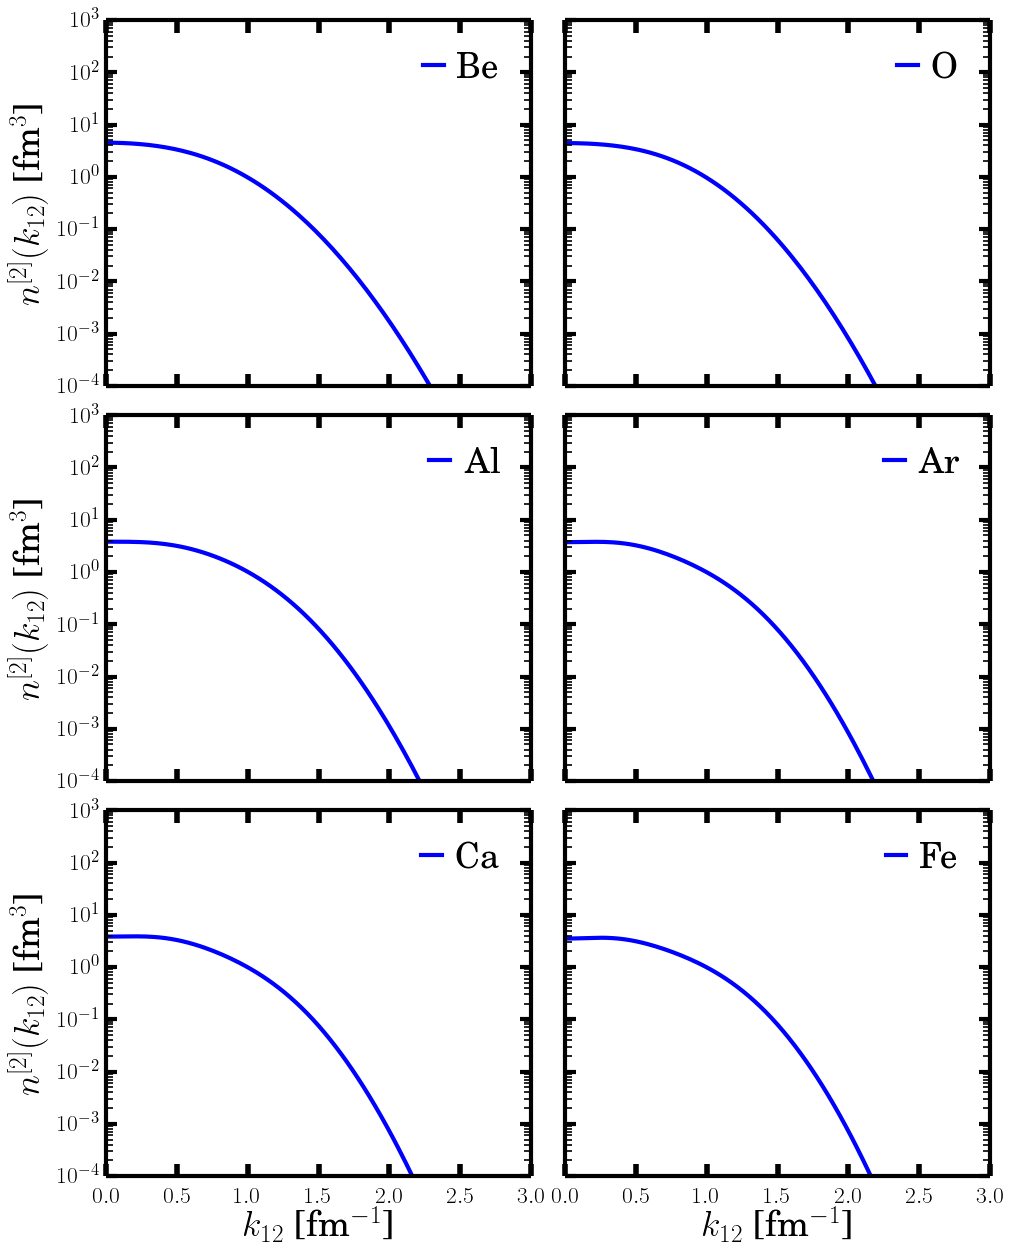
\includegraphics[scale=0.6]{multi_tb_rel.png}
\caption{$n^{[2]}(k_{12})$ voor $\nuclide[9][4]{Be}, \nuclide[16][8]{O}, \nuclide[27][13]{Al},\nuclide[40][18]{Ar},\nuclide[40][20]{Ca},\nuclide[56][26]{Fe}$. Alle distributies zijn genormeerd op \'{e}\'{e}n.}
\label{fig:twoparticledistr}
\end{figure}



\appendix

\section{Conventies Tweede kwantisatie}
We schrijven de toestandsvector van een kern in tweede kwantisatie als 
\begin{equation}
\ket{n_1, n_2, n_3 , \ldots}.
\end{equation}
$n_\alpha$ is het aantal deeltjes in het \'{e}\'{e}ndeeltjes orbitaal $u_\alpha$.
Creatie- en annihilatieoperatoren worden respectievelijk gedefini\"{e}rd als  $c^\dagger_\alpha$ en  $c_\alpha$. De creatieoperator $c^\dagger_\alpha$ voegt \'{e}\'{e}n deeltje toe aan een \'{e}\'{e}ndeeltjes orbitaal $u_\alpha$  en $c_\alpha$ verwijdert \'{e}\'{e}n deeltje uit dit orbitaal:
\begin{align}
c^\dagger_\alpha\ket{n_1, n_2, \ldots, n_i, \ldots} & = \left(\mathds{1} \otimes \mathds{1} \otimes \cdots \otimes c^\dagger_\alpha \otimes  \cdots \otimes \mathds{1} \right) \ket{n_1} \otimes \ket{n_2} \otimes \cdots \otimes \ket{n_\alpha} \otimes \cdots \\
& = (-1)^{s_\alpha}\ket{n_1} \otimes \ket{n_2} \otimes \cdots \otimes c^\dagger_\alpha \ket{n_\alpha} \otimes \cdots \\
& = \delta_{0n_\alpha}(-1)^{s_\alpha}\ket{n_1, \ldots, n_{\alpha-1},  n_\alpha+1,  n_{\alpha+1}, \ldots }.
\end{align}
waar
\begin{equation}
s_\alpha= n_1 + n_2 + \ldots + n_{\alpha-1}.
\end{equation}
De kronecker delta zorgt ervoor dat het Pauli-principe voldaan is. De factor $(-1)^{s_\alpha}$ volgt uit de anitcommutatierelaties voor fermionen
\begin{align}
& \{c_\alpha, c^\dagger_\beta \} = \delta_{\alpha \beta} \\
& \{c_\alpha, c_\beta \} =\{c^\dagger_\alpha, c^\dagger_\beta \}  = 0.
\end{align}
De volgende relatie volgt uit dezelfde principes: 
\begin{equation}
c_\alpha \ket{n_1, n_2, \ldots, n_\alpha, \ldots} = \delta_{1n_\alpha}(-1)^{s_\alpha}\ket{n_1, \ldots, n_{\alpha-1},  n_\alpha-1,  n_{\alpha+1}, \ldots }.
\end{equation}
Men kan een teloperator definieren
\begin{equation}
\hat{N} = \sum_\alpha c^\dagger_\alpha c_\alpha
\end{equation}
die eigenwaarden N $\in \mathds{N}$ heeft en waarvan de eigenfuncties golffuncties zijn met een vast aantal deeltjes. Een genormaliseerde veeldeeltjestoestand kan gecre\"{e}rd worden door creatieoperatoren op de grondtoestand te laten inwerken:
\begin{equation}
\ket{n_1, n_2, n_3 , \ldots} = (c^\dagger_1)^{n_1} (c^\dagger_2)^{n_2} \cdots \ket{0}.
\end{equation}
Deze normalisatie is correct voor fermionen en de $n_i$'s zijn 1 of 0. Men kiest een speciefieke volgorde van de \'{e}\'{e}ndeeltjestoestanden ${u_\alpha}$ en houden deze vast.

Men kan een operator definieren die een deeltje cre\"{e}ert op een plaats $\vec{r}$
\begin{align}
\psi^\dagger(\vec{r}) = \sum_\alpha c^\dagger_\alpha  u^*_\alpha(\vec{r}),
\end{align}
met
\begin{equation}
c^\dagger_\alpha = \int d\vec{r} \psi^\dagger(\vec{r}) u^*_\alpha(\vec{r}).
\end{equation}
Men kan de vergelijkingen controleren door een deeltje te cre\"{e}ren in toestand $\alpha$:
\begin{align}
\ket{\alpha} & = \int d\vec{r} u_\alpha(\vec{r}) \ket{\vec{r}} \\
 & = \int d\vec{r} u_\alpha(\vec{r}) \psi^\dagger(\vec{r}) \ket{0} \\
 & = \int d\vec{r} u_\alpha(\vec{r}) \sum_\beta c^\dagger_\beta  u^*_\beta(\vec{r}) \ket{0} \\
 & = c^\dagger_\alpha \ket{0}.
\end{align}
Bij de laatste stap maakten we gebruik van de orthogonaliteit van de \'{e}\'{e}ndeeltjesorbitalen
\begin{equation}
\int d\vec{r} u_\alpha(\vec{r}) u^*_\beta(\vec{r}) = \delta_{\alpha \beta}
\end{equation}
Men heeft ook nog de volgende relaties
\begin{align}
& u_\alpha(\vec{r})  = \braket{\vec{r}|\vec{\alpha}}  \\
& \braket{\vec{r}|\vec{r}^{\ \prime}} = \delta(\vec{r}-\vec{r}^{\ \prime}) \\
& \braket{\vec{r}|\vec{k}} = \frac{1}{(2\pi)^{3/2}} e^{i\vec{k}\cdot \vec{r}} \\
& \braket{\vec{k}|\vec{r}} = \frac{1}{(2\pi)^{3/2}} e^{-i\vec{k}\cdot \vec{r}}.
\end{align}

Nu wordt een genormaliseerde A-deeltjes Focktoestand in eerste kwatisatie  
\begin{equation}
\ket{\vec{r}_1, \vec{r}_2, \ldots, \vec{r}_A } = \frac{1}{\sqrt{N!}} \psi^\dagger(\vec{r}_1) \psi^\dagger(\vec{r}_2) \cdots \psi^\dagger(\vec{r}_A) \ket{0}
\end{equation}
en de golffunctie in de configuratieruimte
\begin{equation}
\braket{\vec{r}_1, \vec{r}_2, \ldots, \vec{r}_A | n_1, n_2, n_3 , \ldots} = \Psi_A(\vec{r}_1, \vec{r}_2, \ldots, \vec{r}_A ).
\end{equation}

\section{Moshinsky Brackets}
\subsection{Recursieve berekening}
Een tweedeeltjes golfunctie in een harmonische oscillator met totaal impulsmoment $\Lambda$  en projectie $M_\Lambda$ heeft een orthogonale transformatie van individuele co\"{o}rdinaten naar relatieve en massacentrumco\"{o}rdinaten, namelijk de Moshinsky transformatie \cite{moshinsky1959transformation}:
\begin{align}
\Ket{n_1l_1n_2l_2;\Lambda M_\Lambda} = \sum_{nl, N\Lambda} \Ket{nlNL;\Lambda M_\Lambda} \Braket{nlNL;\Lambda | n_1l_1n_2l_2;\Lambda}_{MB}.
\end{align}
Men kan de Moshinsky-brakets berekenen volgens de recursieformule \cite{ursescu2005symbolic}:
\begin{multline}\label{recursion}
\Braket{nlNL;\Lambda | n_1+1l_1n_2l_2;\Lambda}_{MB} = \left[(n_1 +1)(n_1 + l_1 + 3/2) \right]^{-1/2} \\  \times \sum_{n^\prime l^\prime N^\prime L^\prime}   \Braket{nlNL;\Lambda | -r^2_1|n^\prime l^\prime N^\prime L^\prime;\Lambda}\Braket{n^\prime l^\prime N^\prime L^\prime;\Lambda | n_1l_1n_2l_2;\Lambda}_{MB}.
\end{multline}
Wegens behoud van energie moet steeds gelden dat $2(n_1+1) + l_1 + 2n_2 + l_2 = 2n + l + 2N + L$. Indien dit niet het geval is, is de Moshisnky-bracket nul. De matrix-elementen in relatie \eqref{recursion} zijn verschillend van nul voor slechts zes tweedeeltjes toestanden $\ket{n^\prime l^\prime N^\prime L^\prime;\Lambda}$. Deze kunnen gevonden worden in Tabel \ref{tab:matrixelements}. Een analoge recursierelatie 
waarbij de index $n_2$ wordt verhoogd krijgen we door in de eerste factor de index te veranderen ($1 \rightarrow 2$) en de laatste vier matrix-elementen, nu van $-r^2_2$, in Tabel \ref{tab:matrixelements} krijgen een minteken.
\begin{table}
    \begin{tabular}{l  l  l  l  l}
    \hline
    $n^\prime$ &  $l^\prime$  &  $N^\prime$  & $L^\prime$   & $\Braket{nlNL;\Lambda | -r^2_1|n^\prime l^\prime N^\prime L^\prime;\Lambda}$ \\ \hline
    $n-1$ & $l$ & $N$ & $L$ & $\frac{1}{2}\left[n\left(n+l+\frac{1}{2} \right) \right]^{1/2}$ \\
    $n$ & $l$ & $N-1$ & $L$ & $\frac{1}{2}\left[N\left(N+L+\frac{1}{2} \right) \right]^{1/2}$ \\
    $n-1$ & $l+1$ & $N-1$ & $L+1$ & $\left[nN\left(l+1\right) \left(L+1\right) \right]^{1/2} (-1)^{\Lambda + L + l} W(l l+1 L L+1; 1 \Lambda)$ \\
    $n-1$ & $l+1$ & $N$ & $L-1$ & $\left[n(N+L+1/2)\left(l+1\right) L \right]^{1/2} (-1)^{\Lambda + L + l} W(l l+1 L L-1; 1 \Lambda)$ \\
    $n$ & $l-1$ & $N-1$ & $L+1$ & $\left[(n+l+1/2)N l\left(L+1\right) \right]^{1/2} (-1)^{\Lambda + L + l} W(l l-1 L L+1; 1 \Lambda)$ \\
    $n$ & $l-1$ & $N$ & $L-1$ &$\left[(n+l+1/2)(N+L+1/2)l L \right]^{1/2} (-1)^{\Lambda + L + l} W(l l-1 L L-1; 1 \Lambda)$ \\
    \hline
    \end{tabular}
    \caption{The matrix elements of $-r^2_1$}
  \label{tab:matrixelements}
\end{table}
Dus kan men $\Braket{nlNL;\Lambda | n_1l_1n_2l_2;\Lambda}_{MB}$ berekenen startend van $\Braket{nlNL;\Lambda | 0l_10l_2;\Lambda}_{MB}$. Een uitdrukking hiervoor kan gevonden worden in \cite{ursescu2005symbolic}:
\begin{multline} \label{eq:start_mosh}
\Braket{nlNL;\Lambda | 0 l_10 l_2;\Lambda}_{MB} \\ = \left[ \frac{l_1! l_2!}{(2l_1)!(2l_2)!} \frac{(2l+1)(2L+1)}{2^{l+L}} \frac{(n+l)!}{n!(2n+2l+1)!} \frac{(N+L)!}{n!(2N+2L+1)!}  \right]^{1/2} \\
\times (-1)^{n+l+L-\Lambda} \sum_x (2x+1) A(l_1 l, l_2 L,x) W(lLl_1 l_2;\Lambda x)
\end{multline}
met 
\begin{multline}
A(l_1 l, l_2 L,x) = \left[ \frac{(l_1+l+x+1)! (l_1 + l -x)!(l_1 + x -l)!}{(l + x-l_1)!} \frac{(l_2+L+x+1)! (l_2 + L -x)!(l_2 + x -L)!}{(L + x-l_2)!} \right]^{1/2} \\ 
\sum_q (-1)^{\frac{l+q-l_1}{2}}  \frac{(l+q-1_1)!}{\left(\frac{(l + q -l_1)}{2}\right)!\left(\frac{(l + l_1-q)}{2}\right)!} \frac{1}{(q-x)! (q+x+)!} \frac{(L+q-l_2)!}{\left(\frac{(L + q -l_2)}{2}\right)!\left(\frac{(L + l_2-q)}{2}\right)!}.
\end{multline}
De sommatie over $q$ is beprerkt tot die positieve waarden van $q$ waarvoor de argumenten van de faculteiten niet-negatief zijn. 
$W(lLL_1 l_2;\Lambda x)$ stelt de Racah W coefficient voor en staat in verband met de Wigner 6-j symbolen:
\begin{equation}
W(lLl_1 l_2;\Lambda x) = (-1)^{l + L + l_1 + l_2} \left\{ \begin{matrix} 
                             l & L & \Lambda \\ 
                            l_2 & l_1 & x
                          \end{matrix} \right\}.
\end{equation}
De restricties voor de sommatie over $x$ in \eqref{eq:start_mosh} worden gegeven door 
\begin{equation}
\begin{matrix}
\abs{l-l_1} \leq x \leq l+l_1 & \abs{L-l_2} \leq x \leq L+l_2.
\end{matrix}
\end{equation}
Deze relaties volgen uit de symmetrie-eigenschappen van het Wigner 6-j symbool. `

\subsection{Eigenschappen}
Moshinsky-brackets hebben de volgende orthogonaliteitsrelaties:
\begin{align}
\sum_{nlNL} \Braket{nlNL;\Lambda | n_1l_1n_2l_2;\Lambda}_{MB} \Braket{nlNL;\Lambda | n^\prime_1l^\prime_1n^\prime_2 l^\prime_2;\Lambda}_{MB} = \delta_{n_1n^\prime_1} \delta_{l_1l^\prime_1}\delta_{n_2n^\prime_2}\delta_{l_2l^\prime_2} \\
\sum_{n_1l_1n_2l_2} \Braket{nlNL;\Lambda | n_1l_1n_2l_2;\Lambda}_{MB} \Braket{n^\prime l^\prime N^\prime L^\prime;\Lambda | n_1l_1n_2l_2;\Lambda}_{MB} = \delta_{n n^\prime} \delta_{l l^\prime}\delta_{N N^\prime}\delta_{L L^\prime} 
\end{align}
De volgende symmetrierelaties gelden:
\begin{align*}
\Braket{nlNL;\Lambda | n_1l_1n_2l_2;\Lambda}_{MB} &= (-1)^{L-\Lambda} \Braket{nlNL;\Lambda | n_2l_2n_1l_1;\Lambda}_{MB} \\
& = (-1)^{l_1-\Lambda} \Braket{NLnl;\Lambda | n_1l_1n_2l_2;\Lambda}_{MB} \\
& = (-1)^{l_1+l} \Braket{NLnl;\Lambda | n_2l_2n_1l_1;\Lambda}_{MB} \\
& = (-1)^{l_2+L} \Braket{n_1l_1n_2l_2;\Lambda | NLnl;\Lambda}_{MB} 
\end{align*}



Het bewijs van bovenstaande relaties kan men vinden in \cite{brody1967tables}.
\bibliographystyle{plain}
\bibliography{moshinsky,symbolic_algorithms_moshinsky,subatomic,argoneutrino,ankowski,qsrc,transformation}
\end{document}





